% Graphic for TeX using PGF
% Title: /home/indenml/code/bachelor_thesis/content/figures/language_spec-erm-geschaeftsobjekt.dia
% Creator: Dia v0.97.3
% CreationDate: Tue Sep 27 11:17:50 2016
% For: indenml
% \usepackage{tikz}
% The following commands are not supported in PSTricks at present
% We define them conditionally, so when they are implemented,
% this pgf file will use them.
\ifx\du\undefined{}
  \newlength{\du}
\fi
\setlength{\du}{15\unitlength}
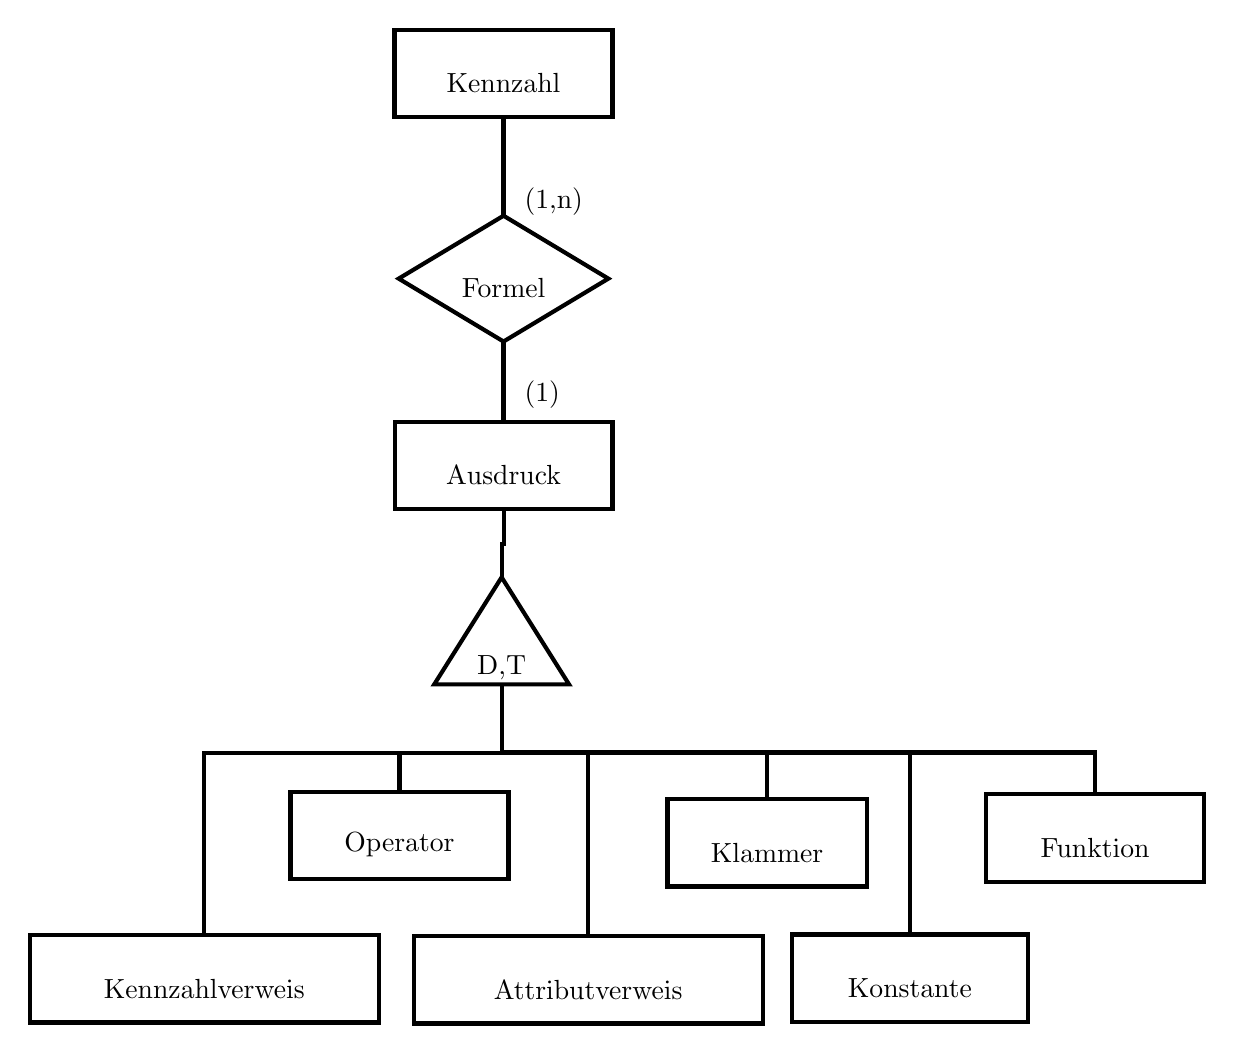
\begin{tikzpicture}
\pgftransformxscale{1.171906}
\pgftransformyscale{-1.171906}
\definecolor{dialinecolor}{rgb}{0.000000, 0.000000, 0.000000}
\pgfsetstrokecolor{dialinecolor}
\definecolor{dialinecolor}{rgb}{1.000000, 1.000000, 1.000000}
\pgfsetfillcolor{dialinecolor}
\definecolor{dialinecolor}{rgb}{1.000000, 1.000000, 1.000000}
\pgfsetfillcolor{dialinecolor}
\fill (14.242400\du,25.644600\du)--(14.242400\du,27.444600\du)--(18.722400\du,27.444600\du)--(18.722400\du,25.644600\du)--cycle;
\pgfsetlinewidth{0.100000\du}
\pgfsetdash{}{0pt}
\pgfsetmiterjoin
\definecolor{dialinecolor}{rgb}{0.000000, 0.000000, 0.000000}
\pgfsetstrokecolor{dialinecolor}
\draw (14.242400\du,25.644600\du)--(14.242400\du,27.444600\du)--(18.722400\du,27.444600\du)--(18.722400\du,25.644600\du)--cycle;
% setfont left to latex
\definecolor{dialinecolor}{rgb}{0.000000, 0.000000, 0.000000}
\pgfsetstrokecolor{dialinecolor}
\node at (16.482400\du,26.744600\du){Kennzahl};
\definecolor{dialinecolor}{rgb}{1.000000, 1.000000, 1.000000}
\pgfsetfillcolor{dialinecolor}
\fill (14.244400\du,33.701100\du)--(14.244400\du,35.501100\du)--(18.724400\du,35.501100\du)--(18.724400\du,33.701100\du)--cycle;
\pgfsetlinewidth{0.100000\du}
\pgfsetdash{}{0pt}
\pgfsetmiterjoin
\definecolor{dialinecolor}{rgb}{0.000000, 0.000000, 0.000000}
\pgfsetstrokecolor{dialinecolor}
\draw (14.244400\du,33.701100\du)--(14.244400\du,35.501100\du)--(18.724400\du,35.501100\du)--(18.724400\du,33.701100\du)--cycle;
% setfont left to latex
\definecolor{dialinecolor}{rgb}{0.000000, 0.000000, 0.000000}
\pgfsetstrokecolor{dialinecolor}
\node at (16.484400\du,34.801100\du){Ausdruck};
\definecolor{dialinecolor}{rgb}{1.000000, 1.000000, 1.000000}
\pgfsetfillcolor{dialinecolor}
\fill (14.329000\du,30.760100\du)--(16.484000\du,29.467100\du)--(18.639000\du,30.760100\du)--(16.484000\du,32.053100\du)--cycle;
\pgfsetlinewidth{0.100000\du}
\pgfsetdash{}{0pt}
\pgfsetmiterjoin
\definecolor{dialinecolor}{rgb}{0.000000, 0.000000, 0.000000}
\pgfsetstrokecolor{dialinecolor}
\draw (14.329000\du,30.760100\du)--(16.484000\du,29.467100\du)--(18.639000\du,30.760100\du)--(16.484000\du,32.053100\du)--cycle;
% setfont left to latex
\definecolor{dialinecolor}{rgb}{0.000000, 0.000000, 0.000000}
\pgfsetstrokecolor{dialinecolor}
\node[anchor=west] at (16.684000\du,29.167100\du){(1,n)};
\definecolor{dialinecolor}{rgb}{0.000000, 0.000000, 0.000000}
\pgfsetstrokecolor{dialinecolor}
\node[anchor=west] at (16.684000\du,33.153100\du){(1)};
\definecolor{dialinecolor}{rgb}{0.000000, 0.000000, 0.000000}
\pgfsetstrokecolor{dialinecolor}
\node at (16.484000\du,30.960100\du){Formel};
\pgfsetlinewidth{0.100000\du}
\pgfsetdash{}{0pt}
\pgfsetmiterjoin
\pgfsetbuttcap
\definecolor{dialinecolor}{rgb}{0.000000, 0.000000, 0.000000}
\pgfsetstrokecolor{dialinecolor}
\draw (16.482400\du,27.444600\du)--(16.482400\du,27.437200\du)--(16.484000\du,27.437200\du)--(16.484000\du,29.467100\du);
\pgfsetlinewidth{0.100000\du}
\pgfsetdash{}{0pt}
\pgfsetmiterjoin
\pgfsetbuttcap
\definecolor{dialinecolor}{rgb}{0.000000, 0.000000, 0.000000}
\pgfsetstrokecolor{dialinecolor}
\draw (16.484000\du,32.053100\du)--(16.483900\du,32.053100\du)--(16.483900\du,33.701100\du)--(16.484400\du,33.701100\du);
\pgfsetlinewidth{0.100000\du}
\pgfsetdash{}{0pt}
\pgfsetdash{}{0pt}
\pgfsetbuttcap
\pgfsetmiterjoin
\pgfsetlinewidth{0.100000\du}
\pgfsetbuttcap
\pgfsetmiterjoin
\pgfsetdash{}{0pt}
\definecolor{dialinecolor}{rgb}{1.000000, 1.000000, 1.000000}
\pgfsetfillcolor{dialinecolor}
\fill (15.059400\du,39.100028\du)--(17.829400\du,39.100028\du)--(16.444400\du,36.900028\du)--cycle;
\definecolor{dialinecolor}{rgb}{0.000000, 0.000000, 0.000000}
\pgfsetstrokecolor{dialinecolor}
\draw (15.059400\du,39.100028\du)--(17.829400\du,39.100028\du)--(16.444400\du,36.900028\du)--cycle;
% setfont left to latex
\definecolor{dialinecolor}{rgb}{0.000000, 0.000000, 0.000000}
\pgfsetstrokecolor{dialinecolor}
\node at (16.444400\du,38.750028\du){D,T};
\definecolor{dialinecolor}{rgb}{1.000000, 1.000000, 1.000000}
\pgfsetfillcolor{dialinecolor}
\fill (26.404400\du,41.356500\du)--(26.404400\du,43.156500\du)--(30.884400\du,43.156500\du)--(30.884400\du,41.356500\du)--cycle;
\pgfsetlinewidth{0.100000\du}
\pgfsetdash{}{0pt}
\pgfsetmiterjoin
\definecolor{dialinecolor}{rgb}{0.000000, 0.000000, 0.000000}
\pgfsetstrokecolor{dialinecolor}
\draw (26.404400\du,41.356500\du)--(26.404400\du,43.156500\du)--(30.884400\du,43.156500\du)--(30.884400\du,41.356500\du)--cycle;
% setfont left to latex
\definecolor{dialinecolor}{rgb}{0.000000, 0.000000, 0.000000}
\pgfsetstrokecolor{dialinecolor}
\node at (28.644400\du,42.456500\du){Funktion};
\definecolor{dialinecolor}{rgb}{1.000000, 1.000000, 1.000000}
\pgfsetfillcolor{dialinecolor}
\fill (12.104400\du,41.306500\du)--(12.104400\du,43.106500\du)--(16.584400\du,43.106500\du)--(16.584400\du,41.306500\du)--cycle;
\pgfsetlinewidth{0.100000\du}
\pgfsetdash{}{0pt}
\pgfsetmiterjoin
\definecolor{dialinecolor}{rgb}{0.000000, 0.000000, 0.000000}
\pgfsetstrokecolor{dialinecolor}
\draw (12.104400\du,41.306500\du)--(12.104400\du,43.106500\du)--(16.584400\du,43.106500\du)--(16.584400\du,41.306500\du)--cycle;
% setfont left to latex
\definecolor{dialinecolor}{rgb}{0.000000, 0.000000, 0.000000}
\pgfsetstrokecolor{dialinecolor}
\node at (14.344400\du,42.406500\du){Operator};
\definecolor{dialinecolor}{rgb}{1.000000, 1.000000, 1.000000}
\pgfsetfillcolor{dialinecolor}
\fill (19.854400\du,41.456500\du)--(19.854400\du,43.256500\du)--(23.949400\du,43.256500\du)--(23.949400\du,41.456500\du)--cycle;
\pgfsetlinewidth{0.100000\du}
\pgfsetdash{}{0pt}
\pgfsetmiterjoin
\definecolor{dialinecolor}{rgb}{0.000000, 0.000000, 0.000000}
\pgfsetstrokecolor{dialinecolor}
\draw (19.854400\du,41.456500\du)--(19.854400\du,43.256500\du)--(23.949400\du,43.256500\du)--(23.949400\du,41.456500\du)--cycle;
% setfont left to latex
\definecolor{dialinecolor}{rgb}{0.000000, 0.000000, 0.000000}
\pgfsetstrokecolor{dialinecolor}
\node at (21.901900\du,42.556500\du){Klammer};
\definecolor{dialinecolor}{rgb}{1.000000, 1.000000, 1.000000}
\pgfsetfillcolor{dialinecolor}
\fill (6.744370\du,44.251500\du)--(6.744370\du,46.051500\du)--(13.919370\du,46.051500\du)--(13.919370\du,44.251500\du)--cycle;
\pgfsetlinewidth{0.100000\du}
\pgfsetdash{}{0pt}
\pgfsetmiterjoin
\definecolor{dialinecolor}{rgb}{0.000000, 0.000000, 0.000000}
\pgfsetstrokecolor{dialinecolor}
\draw (6.744370\du,44.251500\du)--(6.744370\du,46.051500\du)--(13.919370\du,46.051500\du)--(13.919370\du,44.251500\du)--cycle;
% setfont left to latex
\definecolor{dialinecolor}{rgb}{0.000000, 0.000000, 0.000000}
\pgfsetstrokecolor{dialinecolor}
\node at (10.331870\du,45.351500\du){Kennzahlverweis};
\definecolor{dialinecolor}{rgb}{1.000000, 1.000000, 1.000000}
\pgfsetfillcolor{dialinecolor}
\fill (14.634400\du,44.271500\du)--(14.634400\du,46.071500\du)--(21.809400\du,46.071500\du)--(21.809400\du,44.271500\du)--cycle;
\pgfsetlinewidth{0.100000\du}
\pgfsetdash{}{0pt}
\pgfsetmiterjoin
\definecolor{dialinecolor}{rgb}{0.000000, 0.000000, 0.000000}
\pgfsetstrokecolor{dialinecolor}
\draw (14.634400\du,44.271500\du)--(14.634400\du,46.071500\du)--(21.809400\du,46.071500\du)--(21.809400\du,44.271500\du)--cycle;
% setfont left to latex
\definecolor{dialinecolor}{rgb}{0.000000, 0.000000, 0.000000}
\pgfsetstrokecolor{dialinecolor}
\node at (18.221900\du,45.371500\du){Attributverweis};
\definecolor{dialinecolor}{rgb}{1.000000, 1.000000, 1.000000}
\pgfsetfillcolor{dialinecolor}
\fill (22.404400\du,44.241500\du)--(22.404400\du,46.041500\du)--(27.269400\du,46.041500\du)--(27.269400\du,44.241500\du)--cycle;
\pgfsetlinewidth{0.100000\du}
\pgfsetdash{}{0pt}
\pgfsetmiterjoin
\definecolor{dialinecolor}{rgb}{0.000000, 0.000000, 0.000000}
\pgfsetstrokecolor{dialinecolor}
\draw (22.404400\du,44.241500\du)--(22.404400\du,46.041500\du)--(27.269400\du,46.041500\du)--(27.269400\du,44.241500\du)--cycle;
% setfont left to latex
\definecolor{dialinecolor}{rgb}{0.000000, 0.000000, 0.000000}
\pgfsetstrokecolor{dialinecolor}
\node at (24.836900\du,45.341500\du){Konstante};
\pgfsetlinewidth{0.100000\du}
\pgfsetdash{}{0pt}
\pgfsetmiterjoin
\pgfsetbuttcap
\definecolor{dialinecolor}{rgb}{0.000000, 0.000000, 0.000000}
\pgfsetstrokecolor{dialinecolor}
\draw (28.644400\du,41.356500\du)--(28.644400\du,40.500000\du)--(16.444400\du,40.500000\du)--(16.444400\du,39.100028\du);
\pgfsetlinewidth{0.100000\du}
\pgfsetdash{}{0pt}
\pgfsetmiterjoin
\pgfsetbuttcap
\definecolor{dialinecolor}{rgb}{0.000000, 0.000000, 0.000000}
\pgfsetstrokecolor{dialinecolor}
\draw (14.344400\du,41.306500\du)--(14.344400\du,40.506300\du)--(16.444400\du,40.506300\du)--(16.444400\du,39.100028\du);
\pgfsetlinewidth{0.100000\du}
\pgfsetdash{}{0pt}
\pgfsetmiterjoin
\pgfsetbuttcap
\definecolor{dialinecolor}{rgb}{0.000000, 0.000000, 0.000000}
\pgfsetstrokecolor{dialinecolor}
\draw (10.331870\du,44.251500\du)--(10.331870\du,40.512500\du)--(16.444400\du,40.512500\du)--(16.444400\du,39.100028\du);
\pgfsetlinewidth{0.100000\du}
\pgfsetdash{}{0pt}
\pgfsetmiterjoin
\pgfsetbuttcap
\definecolor{dialinecolor}{rgb}{0.000000, 0.000000, 0.000000}
\pgfsetstrokecolor{dialinecolor}
\draw (18.221900\du,44.271500\du)--(18.221900\du,40.512500\du)--(16.444400\du,40.512500\du)--(16.444400\du,39.100028\du);
\pgfsetlinewidth{0.100000\du}
\pgfsetdash{}{0pt}
\pgfsetmiterjoin
\pgfsetbuttcap
\definecolor{dialinecolor}{rgb}{0.000000, 0.000000, 0.000000}
\pgfsetstrokecolor{dialinecolor}
\draw (21.901900\du,41.456500\du)--(21.901900\du,40.501500\du)--(16.444400\du,40.501500\du)--(16.444400\du,39.100028\du);
\pgfsetlinewidth{0.100000\du}
\pgfsetdash{}{0pt}
\pgfsetmiterjoin
\pgfsetbuttcap
\definecolor{dialinecolor}{rgb}{0.000000, 0.000000, 0.000000}
\pgfsetstrokecolor{dialinecolor}
\draw (24.836900\du,44.241500\du)--(24.836900\du,40.512500\du)--(16.444400\du,40.512500\du)--(16.444400\du,39.100028\du);
\pgfsetlinewidth{0.100000\du}
\pgfsetdash{}{0pt}
\pgfsetmiterjoin
\pgfsetbuttcap
\definecolor{dialinecolor}{rgb}{0.000000, 0.000000, 0.000000}
\pgfsetstrokecolor{dialinecolor}
\draw (16.444400\du,36.900028\du)--(16.444400\du,36.212500\du)--(16.484400\du,36.212500\du)--(16.484400\du,35.501100\du);
\end{tikzpicture}
